\subsection{\texttt{naiveBayesKlassifier} class}

The Naive Bayes classifier was implemented in \textsc{Matlab} as a class called \texttt{naiveBayesKlassifier} as to mimic existing \textsc{Matlab} or python libraries. I has two basic methods which correspond to the training and testing steps aforementioned.

\begin{itemize}
	\item Properties	
	\begin{itemize}
		\item \texttt{predictorNames}: names of each predictor.
		\item \texttt{targetName}: name of the target vector.
		\item \texttt{classNames}: the different classes found in the target vector.
		\item \texttt{numObservations}: total number of observations for the training set.
		\item \texttt{categoricalLevels}: levels per predictor represented in categorical form.
		\item \texttt{numericalLevels}: levels per predictor represented in numerical form.
		\item \texttt{numericalPredictor}: numerical matrix containing the numerical representation of the training categorical set.
		\item \texttt{numericalTarget}: numerical representation of the target vector.
		\item \texttt{smoothing}: flag for smoothing (default = YES).
		\item \texttt{priorProbs}: prior probabilities for each class.
		\item \texttt{likelihood}: likelihood values per predictor per level (cell array of dimension k\_classes $\times$ n\_predictors).
	\end{itemize}
	\item Methods
	\begin{itemize}
		\item \texttt{fit(training\_set)}:
		Receives a table object as an input and from this it sets up all the properties of the class
		\item \texttt{predict(test\_set)}:
		Receives a table object as input and uses the probabilities contained  in in \texttt{priorProbs} and \texttt{likelihood} to compute the prediction vector. If a test target vector is also included the corresponding accuracy of the prediction is also computed.
	\end{itemize}
\end{itemize}

When using the whole dataset as training set, we obtain the following:
\begin{lstlisting}[language=MATLAB]
naiveBayesKlassifier with properties:

predictorNames: {'Outlook' 'Temperature' 'Humidity'  'Windy'}
targetName: {'Play'}
classNames: [no    yes]
numObservations: 14
categoricalLevels: {{3x1 cell} {3x1 cell} {2x1 cell}  {2x1 cell}}
numericalLevels: {[3x1 double]  [3x1 double]  [2x1 double]  [2x1 double]}
numericalPredictor: [14x4 double]
numericalTarget: [14x1 double]
smoothing: 'Yes'
priorProbs: [0.3571 0.6429]
likelihood: {2x4 cell}
\end{lstlisting}

Going deeper in some of the priorities we find the mapping of categorical to numerical that yields table \ref{tbl:weather_numerical_dataset}.
\begin{itemize}
	\item \texttt{categoricalLevels} =
	\begin{equation*}
	\left\lbrace 
	\begin{bmatrix} \text{overcast} \\ \text{rainy} \\ \text{sunny} \end{bmatrix},
	\begin{bmatrix} \text{cool} \\ \text{hot} \\ \text{mild} \end{bmatrix},
	\begin{bmatrix} \text{high} \\ \text{normal} \end{bmatrix},
	\begin{bmatrix} \text{FALSE} \\ \text{TRUE} \end{bmatrix} 
	\right\rbrace 
	\end{equation*} 
	\item \texttt{numericalLevels} =
	\begin{equation*}
	\left\lbrace 
	\begin{bmatrix} 1 \\ 2 \\ 3 \end{bmatrix},
	\begin{bmatrix} 1 \\ 2 \\ 3 \end{bmatrix},
	\begin{bmatrix} 1 \\ 2 \end{bmatrix},
	\begin{bmatrix} 1 \\ 2 \end{bmatrix}
	\right\rbrace 
	\end{equation*} 
\end{itemize}

\begin{table}[]
	% increase table row spacing, adjust to taste
	\renewcommand{\arraystretch}{1.3}
	% if using array.sty, it might be a good idea to tweak the value of
	% \extrarowheight as needed to properly center the text within the cells
	\caption{Weather numerical dataset}
	\label{tbl:weather_numerical_dataset}
	\centering
	% Some packages, such as MDW tools, offer better commands for making tables
	% than the plain LaTeX2e tabular which is used here.
	\begin{tabular}{|c|c|c|c||c|}
		\hline
		Outlook  & Temperature & Humidity & Windy & Play \\ \hline \hline
		1 &  2 &  1  &  1 & 2 \\ \hline
		1 &  1 &  2  &  2 & 2 \\ \hline
		1 &  3 &  1  &  2 & 2 \\ \hline
		1 &  2 &  2  &  1 & 2 \\ \hline
		2 &  3 &  1  &  1 & 2 \\ \hline
		2 &  1 &  2  &  1 & 2 \\ \hline
		2 &  1 &  2  &  2 & 1 \\ \hline
		2 &  3 &  2  &  1 & 2 \\ \hline
		2 &  3 &  1  &  2 & 1 \\ \hline
		3 &  2 &  1  &  1 & 1 \\ \hline
		3 &  2 &  1  &  2 & 1 \\ \hline
		3 &  3 &  1  &  1 & 1 \\ \hline
		3 &  1 &  2  &  1 & 2 \\ \hline
		3 &  3 &  2  &  2 & 2 \\ \hline
	\end{tabular}
\end{table}

The \texttt{likelihood} cell array contains all the likelihood values arranged in a 3D structure where the first dimension corresponds to the $k$-th class, the second dimension corresponds to the $n$-th predictor and the third dimension corresponds to the level.
\begin{table}[]
	% increase table row spacing, adjust to taste
	\renewcommand{\arraystretch}{1.3}
	% if using array.sty, it might be a good idea to tweak the value of
	% \extrarowheight as needed to properly center the text within the cells
	\caption{Likelihood cell array}
	\label{tbl:cond_probs_array}
	\centering
	% Some packages, such as MDW tools, offer better commands for making tables
	% than the plain LaTeX2e tabular which is used here.
	\begin{tabular}{|c||c|c|c|c|}
		\hline
		& Outlook  & Temperature & Humidity & Windy \\ \hline \hline
		no  & $\begin{bmatrix} 0.1250 \\ 0.3750 \\ 0.5000 \end{bmatrix}$ &  
		      $\begin{bmatrix} 0.2500 \\ 0.3750 \\ 0.3750 \end{bmatrix}$ & 
		      $\begin{bmatrix} 0.7143 \\ 0.2857 \end{bmatrix}$ &  
		      $\begin{bmatrix} 0.4286 \\ 0.5714 \end{bmatrix}$ \\ \hline
		yes & $\begin{bmatrix} 0.4167 \\ 0.3333 \\ 0.2500 \end{bmatrix}$ &  
			  $\begin{bmatrix} 0.3333 \\ 0.2500 \\ 0.4167 \end{bmatrix}$ & 
			  $\begin{bmatrix} 0.3636 \\ 0.6364 \end{bmatrix}$ &  
			  $\begin{bmatrix} 0.6364 \\ 0.3636 \end{bmatrix}$ \\ \hline
	\end{tabular}
\end{table}

\subsection{Splitting dataset into training and test sets}

Splitting the available data into training and test subsets is a common practice in machine learning. The process of splitting is preferably done randomly, that is, selecting certain random observations for the training split and leaving the rest for testing. Suitable training:testing ratios range from 70:30 to 80:20

A \textsc{Matlab} function was developed for this purpose.
\begin{lstlisting}
[train, test] = train_test_split(data, train_size)
\end{lstlisting}

This function returns two vectors containing indices for the training and testing subsets accordingly. The parameter \texttt{train\_size}  must be a number between $0.0$ and $1.0$ and represent the proportion of the dataset to include in the training split.

\subsection{Testing classifier using random splitting}

We can now proceed to run several tests by randomly splitting the dataset multiple times and run an accuracy analysis. 
\begin{figure}[h]
	\centering
	\begin{subfigure}{.45\textwidth}
		\centering
		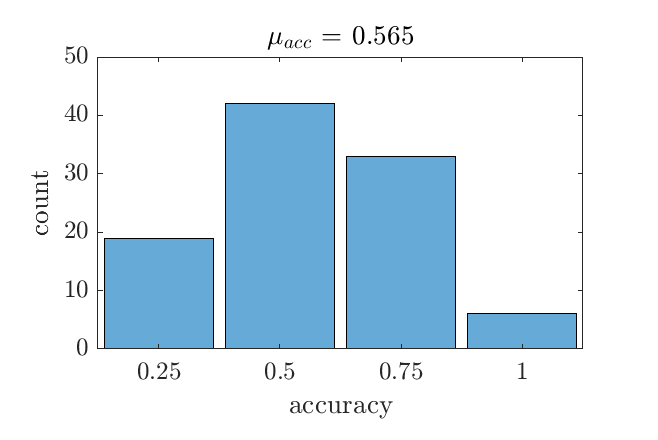
\includegraphics[width=0.9\textwidth]{100iters_random.eps}
		\caption{100 iterations}
		\label{fig:100iters_random}
	\end{subfigure}
	\begin{subfigure}{.45\textwidth}
		\centering
		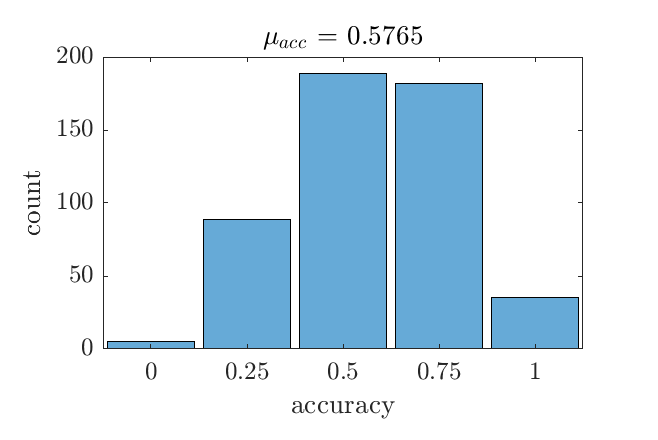
\includegraphics[width=0.9\textwidth]{500iters_random.eps}
		\caption{500 iterations}
		\label{fig:500iters_random}
	\end{subfigure}
	\begin{subfigure}{.45\textwidth}
		\centering
		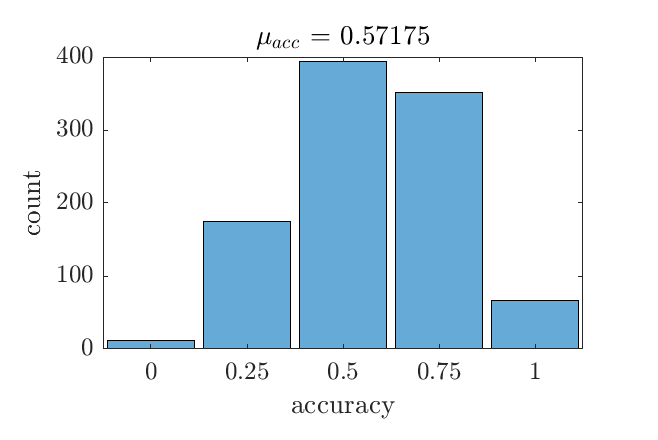
\includegraphics[width=0.9\textwidth]{1000iters_random.eps}
		\caption{1000 iterations}
		\label{fig:1000iters_random}
	\end{subfigure}
	\caption{Performance analysis with random splitting}
	\label{fig:random_splitting}
\end{figure}

The train size is 70\% of the overall data, which translates into 10 observations for the training split and 4 for the testing split. We're interested in the average of accuracy but also in visualizing the results of the several tests conducted. A histogram plot is a powerful visualization tool for this.
\begin{lstlisting}[caption=Simple script for testing classifier]
rng default     % for reproducibility
iters = 100;    % number of iterations
nBK = naiveBayesKlassifier();

for i = 1:iters
	[train_idx, test_idx] = ...
		train_test_split(weather, 0.70);
	
	train_set = weather(train_idx, :);
	nBK.fit(train_set);
	
	test_set = weather(test_idx, :);
	[y_pred, accuracy, ~] = nBK.predict(test_set);
	% analyze results
end
\end{lstlisting}

Results shown in figure \ref{fig:random_splitting} show that the mean accuracy ($\mu_{acc}$) lies around 57\%. Moreover, from the histogram we observe that we have all possible error combinations, that is, we have cases where we get 0\% accuracy going all the way up to 100\%, specially when using a large number of iterations.

\subsection{Stratified splitting}

The results obtained so far are quite disappointing. Since there are no parameters to tune in a Naive Bayes classifier, we proceed to improve the way we split data. When using simple random permutation we're prone to highly unbalanced training and testing splits.

Stratification is the process of dividing members of a population into homogeneous groups before sampling. In machine learning, stratified sampling is used to preserve the percentage of samples for each class \cite{scikit-learn}.
Given the properties of the weather dataset, if we want a 70:30 ratio we'll have:
\begin{itemize}
	\item Training split:
	\begin{itemize}
		\item 4 random observations of the \textit{no} class
		\item 6 random observations of the \textit{yes} class
	\end{itemize}
	\item Test split:
	\begin{itemize}
		\item 1 random observations of the \textit{no} class
		\item 3 random observations of the \textit{yes} class
	\end{itemize}
\end{itemize}

A similar function to \texttt{train\_test\_split} was created but now the output indices will respect the rule for preserving the percentage of samples for each class. 
\begin{lstlisting}
[train, test] = stratified_split(data, train_size)
\end{lstlisting}

\subsection{Testing classifier using stratified splitting}
\begin{figure}[t]
	\centering
	\begin{subfigure}{.45\textwidth}
		\centering
		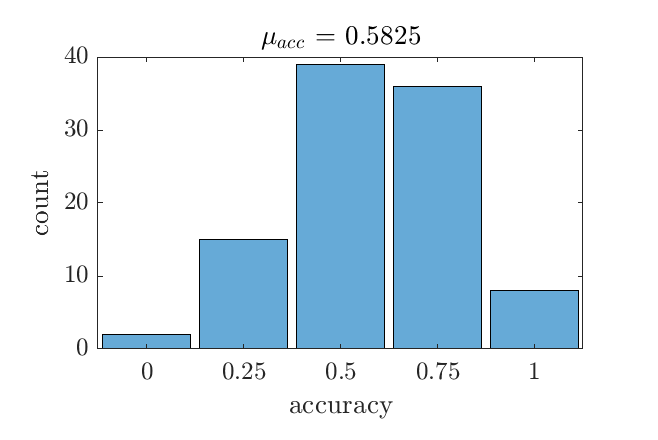
\includegraphics[width=0.9\textwidth]{100iters_stratified.eps}
		\caption{100 iterations}
		\label{fig:100iters_stratified}
	\end{subfigure}
	\begin{subfigure}{.45\textwidth}
		\centering
		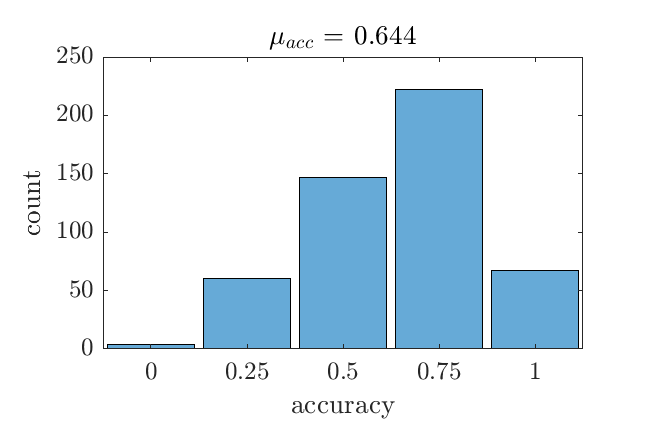
\includegraphics[width=0.9\textwidth]{500iters_stratified.eps}
		\caption{500 iterations}
		\label{fig:500iters_stratified}
	\end{subfigure}
	\begin{subfigure}{.45\textwidth}
		\centering
		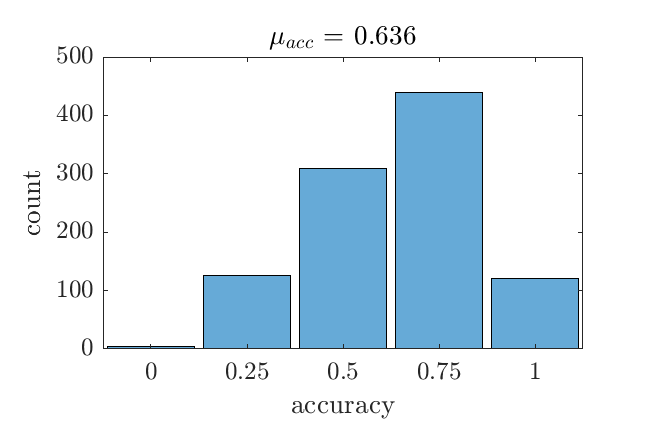
\includegraphics[width=0.9\textwidth]{1000iters_stratified.eps}
		\caption{1000 iterations}
		\label{fig:1000iters_stratified}
	\end{subfigure}
	\caption{Performance analysis with stratified splitting}
	\label{fig:stratified_splitting}
\end{figure}

Same procedure as before was followed with the exception of the function used to split the data. Better results were achieved although we still have cases of 0\% and 100\% accuracy as seen in figure \ref{fig:stratified_splitting}.

When using only 100 iterations the difference is not noticeable. Only when we increase the number of iterations we start appreciating a change in the histogram bar plot shape.


